\documentclass[a4paper,12pt]{article}

\usepackage{tabularx} % Для автоподгона ширины
\usepackage{booktabs} % Для красивых линий \toprule, \midrule, \bottomrule
\usepackage[T2A]{fontenc}
\usepackage[utf8]{inputenc}
\usepackage[russian]{babel}
\usepackage{amsmath, amssymb}
\usepackage{graphicx}
\usepackage{geometry}
\usepackage{booktabs}
\geometry{left=30mm,right=15mm,top=20mm,bottom=20mm}
\usepackage{parskip}

\title{\textbf{Работа 1. Количественные методы в биохимии}}\\


\begin{document}

\maketitle

\section*{Опыт 1. }

 

Выполнено, далее фотоотчет:
\newpage 
\section*{Опыт 2. Свойства буферных растворов}

\subsection*{Теоретическая часть}

Буферными называют растворы, способные сохранять практически постоянное значение $\text{pH}$ при добавлении небольших количеств сильных кислот или оснований, а также при разбавлении.

Состав кислотно-основных буферных растворов описывается уравнением Хендерсона--Хассельбальха:
\begin{equation}
\text{pH} = \text{p}K_a + \lg \frac{[\text{Основание}]}{[\text{Кислота}]}
\end{equation}

В случае Tris-буфера (трис(гидроксиметил)аминометан):
\begin{itemize}
    \item \textbf{Слабое основание:} сопряженное Tris-основание ($\text{Tris}$).
    \item \textbf{Сопряженная кислота:} сопряженная солянокислая соль ТРИС ($\text{Tris}\cdot\text{HCl}$ / $\text{Tris-H}^+$).
\end{itemize}

Важнейшими характеристиками буферной системы являются буферная емкость и способность поддерживать стабильность $\text{pH}$ при добавлении титрантов ($\text{HCl}$, $\text{NaOH}$) и изменении концентрации.

\subsection*{Методика эксперимента}

\begin{enumerate}
    \item \textbf{Приготовление буфера:} К исходному 100~мМ раствору Tris по каплям добавляют раствор 2~М $\text{HCl}$, постоянно перемешивая и измеряя $\text{pH}$, до достижения значения $\text{pH} = 7{,}5$.
    \item \textbf{Исследование буферных свойств:}
    \begin{itemize}
        \item В пробирку помещают 10~мл приготовленного Tris-буфера ($\text{pH} = 7{,}5$).
        \item Используя пипетку (объем одной капли берем $ 50$ мкл), добавляют по 1 капле 0,1~М раствора $\text{HCl}$, перемешивают и замеряют $\text{pH}$ после каждой капли (всего $N = 0\dots10$ кап.).
        \item Повторяют аналогичное титрование 0,1~М раствором $\text{NaOH}$.
    \end{itemize}
    \item \textbf{Контрольный опыт:} Повторяют те же процедуры титрования (0,1~М $\text{HCl}$ и 0,1~М $\text{NaOH}$) для 10~мл дистиллированной воды.
\end{enumerate}

\newpage
\subsection*{Результаты измерений}

\begin{table}[h!]
\centering
\caption{Изменение $\text{pH}$ воды и Tris-буфера при добавлении каплями $\text{HCl}$ и $\text{NaOH}$}
\vspace{0.2cm}
\begin{tabular}{|c|c|c|c|c|}
\hline
\textbf{\begin{tabular}[c]{@{}c@{}}Капли,\\ $N$\end{tabular}} & 
\textbf{\begin{tabular}[c]{@{}c@{}}$\text{pH}$ воды +\\ 0{,}1M HCl\end{tabular}} & 
\textbf{\begin{tabular}[c]{@{}c@{}}$\text{pH}$ буфера +\\ 0{,}1M HCl\end{tabular}} & 
\textbf{\begin{tabular}[c]{@{}c@{}}$\text{pH}$ воды +\\ 0{,}1M NaOH\end{tabular}} & 
\textbf{\begin{tabular}[c]{@{}c@{}}$\text{pH}$ буфера +\\ 0{,}1M NaOH\end{tabular}} \\ \hline
0  & 6{,}72 & 7{,}50 & 6{,}72  & 7{,}55 \\ \hline
1  & 3{,}07 & 7{,}49 & 10{,}00 & 7{,}57 \\ \hline
2  & 2{,}93 & 7{,}46 & 10{,}85 & 7{,}58 \\ \hline
3  & 2{,}79 & 7{,}44 & 11{,}15 & 7{,}59 \\ \hline
4  & 2{,}68 & 7{,}42 & 11{,}25 & 7{,}60 \\ \hline
5  & 2{,}61 & 7{,}40 & 11{,}41 & 7{,}61 \\ \hline
6  & 2{,}52 & 7{,}38 & 11{,}43 & 7{,}62 \\ \hline
7  & 2{,}48 & 7{,}36 & 11{,}49 & 7{,}64 \\ \hline
8  & 2{,}42 & 7{,}33 & 11{,}54 & 7{,}65 \\ \hline
9  & 2{,}41 & 7{,}31 & 11{,}60 & 7{,}67 \\ \hline
10 & 2{,}40 & 7{,}30 & 11{,}64 & 7{,}69 \\ \hline
\end{tabular}
\end{table}

По полученным экспериментальным данным и теоретическим расчетам, мы построили графики зависимости pH растворов от количества капель 0.1 M NaOH и 0.1 M HCl.

\begin{figure}[h]
  \centering
  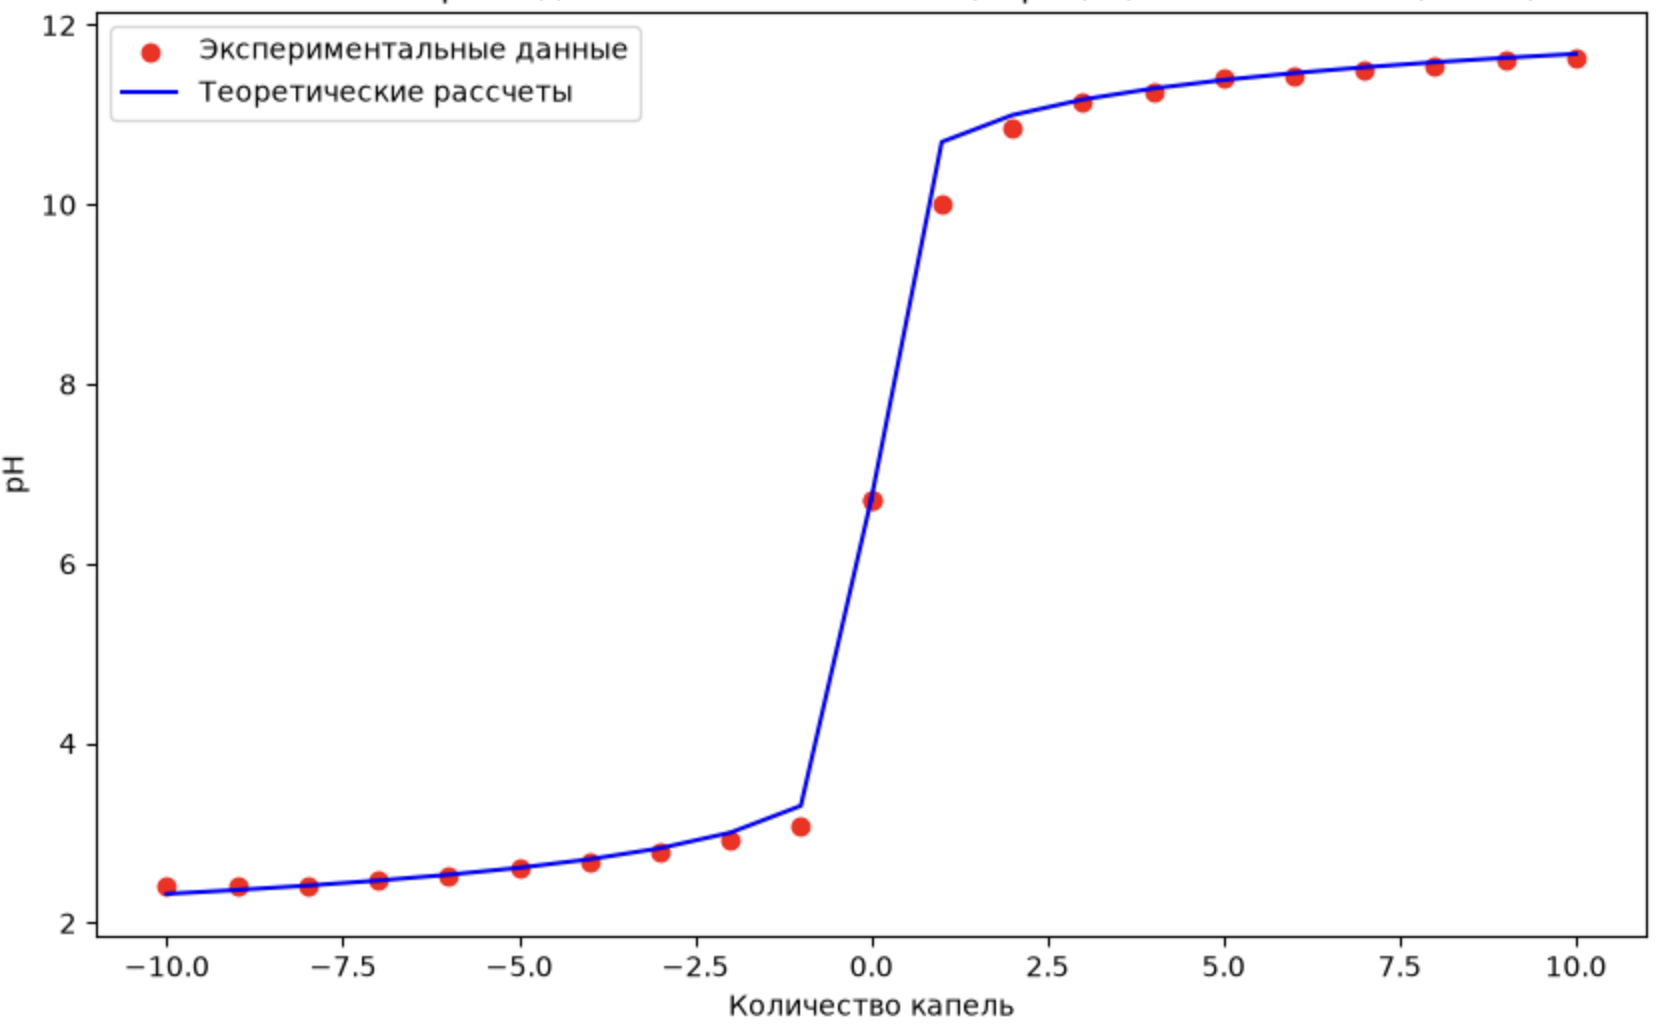
\includegraphics[width=0.8\textwidth]{h2o.png}
  \caption{Зависимость pH воды от кол-ва капель HCl(отриц N) и NaOH(пол N)}
  \label{fig:myimage}
\end{figure}

Теоретические рассчеты неплохо описывают экспериментально полученные данные. В случае воды при добавлении одной капли щелочи или кислоты pH мгновенно сильно меняется (так как появляется большая концентрация $\text{H}^+$ и $\text{OH}^-$), после чего практически не изменяется так как объем добавляемых капель крайне мал по сравнению с изначльным объемом. В случае буфера зависимость немного сложнее. При pH = pKa буферная емкость наибольшая, то есть 'ответ' на добавление кислот и оснований наименьший. Изначальный буфер находился при pH = 7.525 и соотвественно должен быть к кислотам более чувствительным, чем к основаниям, так как находится левее от зоны с наибольшей буферной емкостью. Эта зависимость впринципе и подтверждается на экспериментальных данных.

\begin{figure}[h]
  \centering
  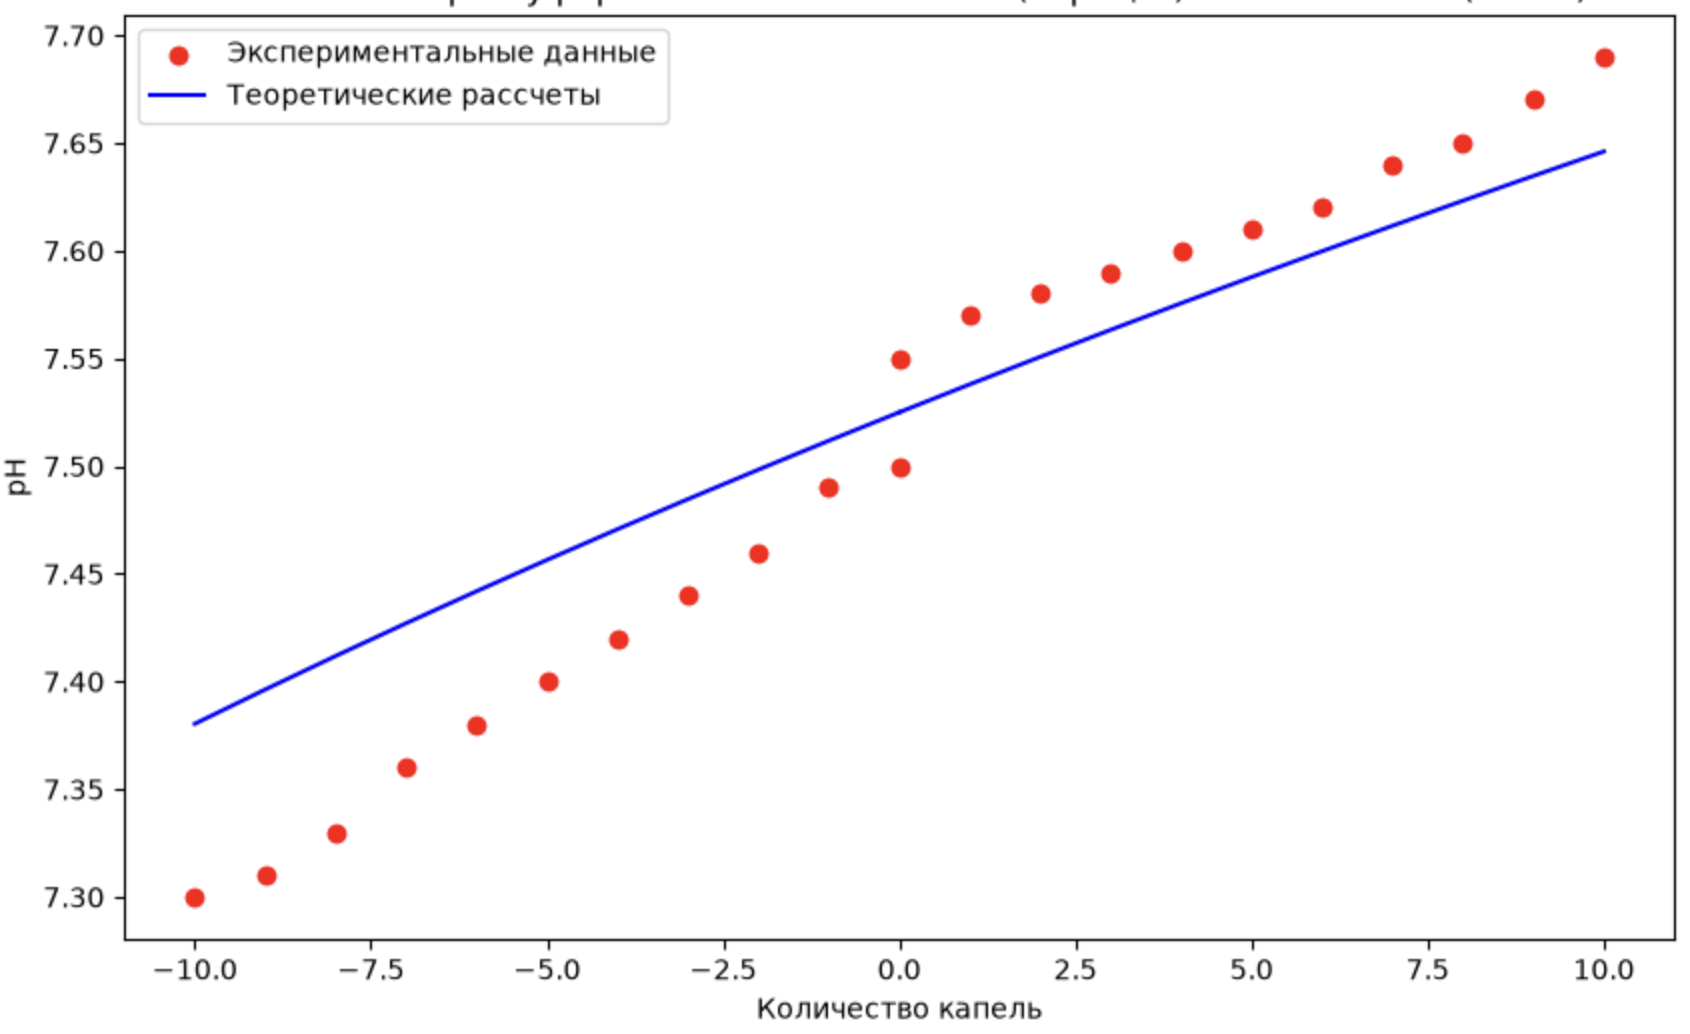
\includegraphics[width=0.75\textwidth]{buf.png}
  \caption{Зависимость pH буфера от кол-ва капель HCl(отриц N) и NaOH(пол N)}
  \label{fig:myimage}
\end{figure}


\begin{figure}[h]
  \centering
  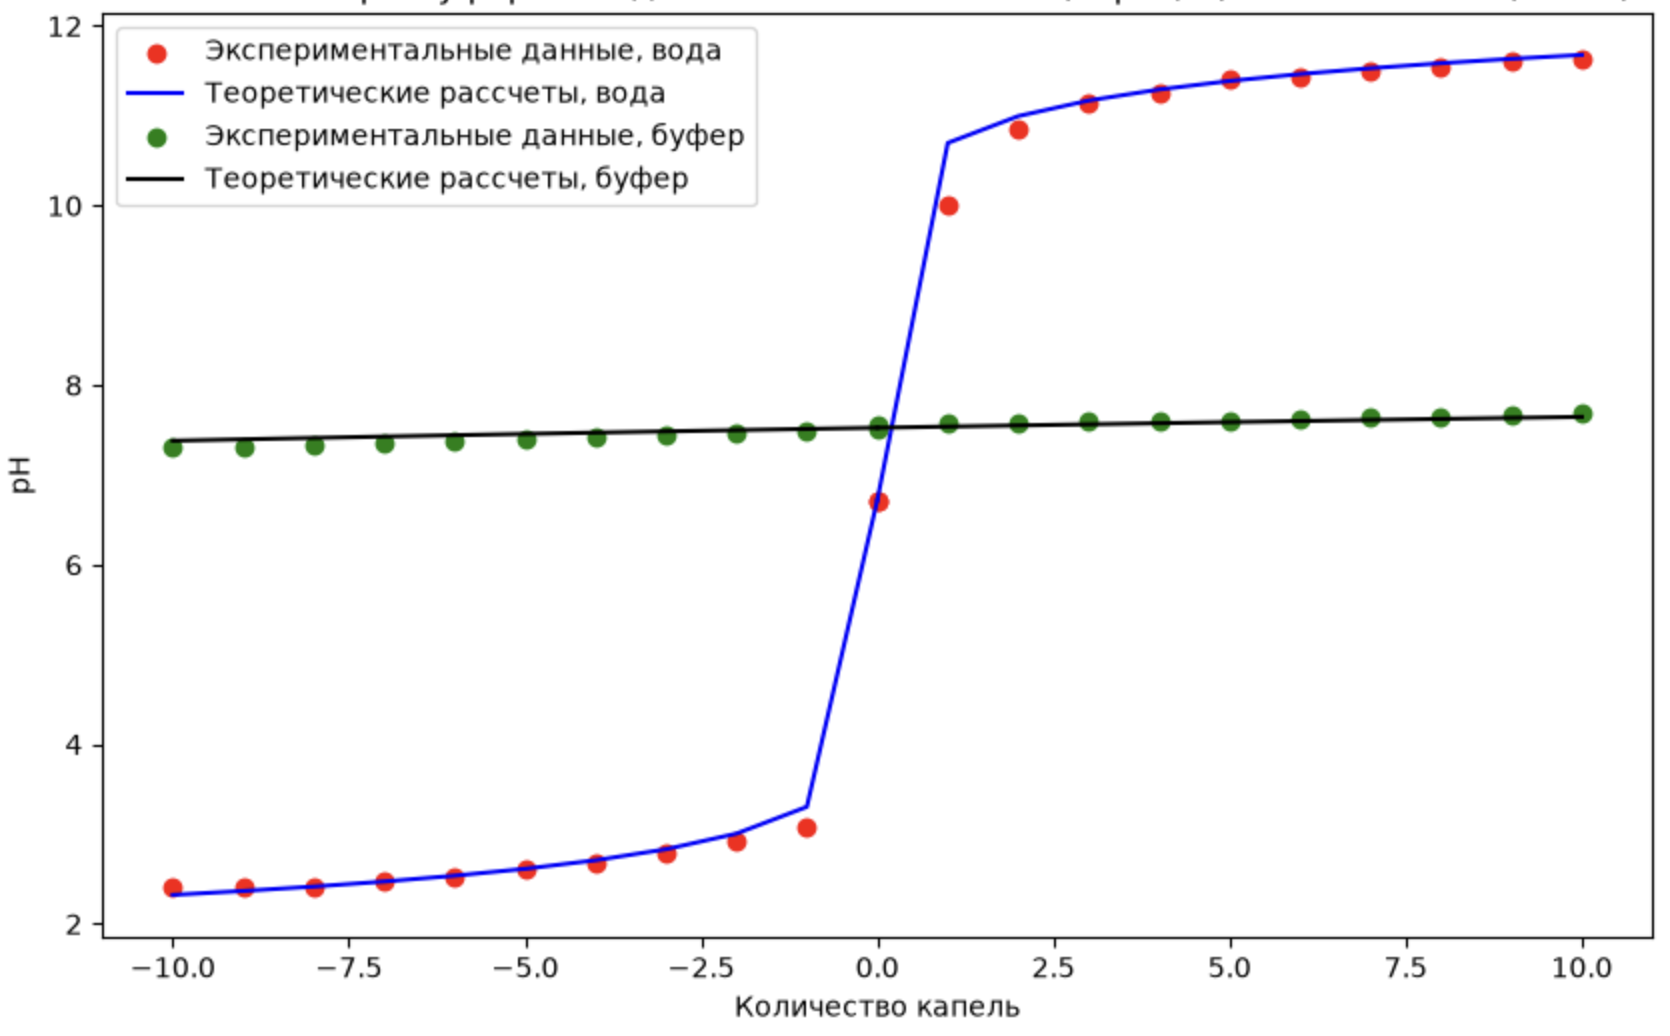
\includegraphics[width=0.75\textwidth]{buf+h20.png}
  \caption{Зависимость pH буфера и воды от кол-ва капель HCl(отриц N) и NaOH(пол N)}
  \label{fig:myimage}
\end{figure}

Ключевыми характеристиками для буфера также являются: 
\begin{itemize}
    \item Буферная емкость. Она отвечает за то, насколько раствор буфера устойчив к добавлению сильных кислот и оснований. К примеру, буферы для клеток должны обладать высокой буферной емкостью, чтобы оптимальный pH не изменялся сильно из-за образующихся при росте и работе бактерий соединений.
    \item Ионная сила. Варьируя концентрацию соли и кислоты (но при этом сохряняя их соотношение) можно сделать серию буферов с одинаковым pH, но с разной ионной силой. К примеру, это может быть важно для выделения каких-то белков или других макромолекул.
\end{itemize}

\newpage

\section*{Опыт 3. }


\end{document}
